\documentclass[openany]{thesisclass}



% ----------------------------------------------------------------
% Thesis - Main document
% ----------------------------------------------------------------

%\usepackage[enlish]{babel}
\usepackage{csquotes}
\usepackage{booktabs}






%% ---------------------------------
%% |      Additional packages      |
%% ---------------------------------
%% 

\usepackage{graphicx}
\DeclareGraphicsExtensions{.pdf,.png,.jpg}
\graphicspath{{./figures/}} %Use curly braces for each path to add and don't forget trailing slash '/'
% \usepackage{epstopdf} %Nice to automatically convert eps figures to pdf format  (from inkscape, etc)






\usepackage[backend=biber,style=authoryear,sorting=ynt]{biblatex}
\bibliography{thesis} 
%\bibliographystyle{ieeetr}



%% ---------------------------------
%% | Needed for the List of Abbreviations |
%% ---------------------------------
\usepackage{nomencl}
\usepackage{lmodern}
\usepackage{listings}
\usepackage{chngcntr}
\usepackage{amsmath}
\usepackage{mathtools}
\usepackage[utf8]{inputenc}
\usepackage[T1]{fontenc}
\renewcommand{\nomname}{Definitionen und Abkürzungen}
\setlength{\nomlabelwidth}{.40\hsize}
\renewcommand{\nomlabel}[1]{#1 \dotfill}
\setlength{\nomitemsep}{-\parsep}
\makenomenclature
\usepackage[normalem]{ulem}
\newcommand{\markup}[1]{\uline{#1}}
\makeatletter
\renewcommand*\env@matrix[1][*\c@MaxMatrixCols c]{%
  \hskip -\arraycolsep
  \let\@ifnextchar\new@ifnextchar
  \array{#1}}
\makeatother

\nomenclature{}{}




%% ---------------------------------
%% | Information about the thesis  |
%% ---------------------------------

% uncomment one of the following, according to your thesis
%\newcommand{\mytype}{Bachelor's Thesis} 
%\newcommand{\mytype}{Master's Thesis}
\newcommand{\mytype}{Assignment two of three}

\newcommand{\myname}{Andreas Wenger | Vinzenz Götz}
\newcommand{\matricle}{44267018 | 25173223}
\newcommand{\mytitle}{Numerical model of one-dimensional, transient heat conduction in a fin}
\newcommand{\myinstitute}{}


\newcommand{\reviewerone}{Prof. Roberto Nunhez}

\newcommand{\submissiontime}{WS 23/24}

%% -------------------------------
%% |  Information for PDF file   |
%% -------------------------------
\hypersetup{
 pdfauthor={\myname},
 pdftitle={\mytitle},
 pdfsubject={\mytype},
 pdfkeywords={\mytype, }
}

%% -------------------------------
%% |  settings for code listings   |
%% -------------------------------
\usepackage{xcolor}

\definecolor{codegreen}{rgb}{0,0.6,0}
\definecolor{codegray}{rgb}{0.5,0.5,0.5}
\definecolor{codepurple}{rgb}{0.58,0,0.82}
\definecolor{backcolour}{rgb}{0.95,0.95,0.92}

\lstdefinestyle{mystyle}{
    backgroundcolor=\color{backcolour},   
    commentstyle=\color{codegreen},
    keywordstyle=\color{magenta},
    numberstyle=\tiny\color{codegray},
    stringstyle=\color{codepurple},
    basicstyle=\ttfamily\footnotesize,
    breakatwhitespace=false,         
    breaklines=true,                 
    captionpos=b,                    
    keepspaces=true,                 
    numbers=left,                    
    numbersep=5pt,                  
    showspaces=false,                
    showstringspaces=false,
    showtabs=false,                  
    tabsize=2
}

\lstset{style=mystyle}


%% --------------------------------
%% | Settings for word separation |
%% --------------------------------
% Describe separation hints here:
\hyphenation{
opos-sum
he-lio-trope
}


%% ------------------------
%% |    Including files   |
%% ------------------------
% Only files listed here will be included!
% Userful command for partially translating the document (for bug-fixing e.g.)
\renewcommand{\deg}{^{\circ}}
%%%%%%%%%%%%%%%%%%%%%%%%%%%%%%%%%
%% Here, main documents begins %%
%%%%%%%%%%%%%%%%%%%%%%%%%%%%%%%%%
\begin{document}

\frontmatter
%% titlepage.tex
%%

% coordinates for the bg shape on the titlepage
\newcommand{\diameter}{20}
\newcommand{\xone}{-15}
\newcommand{\xtwo}{160}
\newcommand{\yone}{15}
\newcommand{\ytwo}{-253}

\begin{titlepage}
% bg shape
\begin{tikzpicture}[overlay]
\draw[color=gray]  
 		 (\xone mm, \yone mm)
  -- (\xtwo mm, \yone mm)
 arc (90:0:\diameter pt) 
  -- (\xtwo mm + \diameter pt , \ytwo mm) 
	-- (\xone mm + \diameter pt , \ytwo mm)
 arc (270:180:\diameter pt)
	-- (\xone mm, \yone mm);
\end{tikzpicture}
	\begin{textblock}{10}[0,0](4,2.5)
		
\includegraphics[width=.3\textwidth]{logos/HM_logo.jpg}
	\end{textblock}
	\begin{textblock}{10}[0,0](11,2.5)
			\end{textblock}
	\changefont{ppl}{m}{n}	% helvetica	(phv), % IM Style: palatino (ppl) 
	\vspace*{3.5cm}
	\begin{center}
		\Huge{\mytitle}\\
		\rule{0.05\textwidth}{0.5pt}\\
		\vspace*{2cm}
		\Large{
			\mytype
		}\\
		\vspace*{1cm}
		\huge{\myname}\\
			\Large{\matricle}\\
		\vspace*{1cm}
		\Large{
			\myinstitute
		}
	\end{center}
	\vspace*{1.5cm}
\Large{
\begin{center}
\begin{tabular}[ht]{l c l}
  % Gutachter sind die Professoren, die die Arbeit bewerten. 
  %\iflanguage{english}{Reviewer}{Erstgutachter}: & \hfill  & \reviewerone\\
  & \reviewerone\\
  %Second Supervisor: & \hfill  & \advisortwo\\
  % IM: No second advisor
  % Der zweite betreuende Mitarbeiter kann weggelassen werden. 
\end{tabular}
\end{center}
}


\vspace{1.5cm}
\begin{center}
\large{\submissiontime}
% \iflanguage{english}{Duration:}{Bearbeitungszeit:} \timestart \hspace*{0.25cm}
% -- \hspace*{0.25cm} 
% \timeend}
\end{center}


\begin{textblock}{10}[0,0](4,16.8)
\tiny{ 
	Hochschule für angewandte Wissenschaften München
}
\end{textblock}

\begin{textblock}{10}[0,0](14,16.75)
\large{
	\textbf{www.HM.edu} 
}
\end{textblock}

\end{titlepage}

\pagenumbering{roman}

%\chapter*{Disclaimer}
\addcontentsline{toc}{chapter}{Disclaimer} 
%



\noindent This report was written in \LaTeX. The basic template for it was found on Overleaf and was made available by Martin Knaebele~\cite{template}. It was modified by me to fit the needs of this report.

\noindent All Definitions and Abbreviations in the Definitions and Abbreviations section are directly cited from CS-25 unless stated otherwise.

\noindent This report does not claim completeness nor is it legally binding. For legally binding text, please refer directly to CS 25.1309.


%\chapter*{Abstract}
\addcontentsline{toc}{chapter}{Abstract} 
%
The following report deals with CS 25.1309 and methods of complying with it. The methods and proceedings are dealt with in ARP4761 and ARP4754 which are themselves mentioned in CS 25.1309 as a reference and are summarized in this report. 


% ISSD Style: No additional blank page
% \blankpage


%% -------------------
%% |   Directories   |
%% -------------------
\tableofcontents

% ISSD Style: No additional blank page
% \blankpaage

% You may elect not to include a list of figures, list of tables and list of abbreviations, if the work is a seminar thesis (comment out the following)
\listoffigures \addcontentsline{toc}{chapter}{Figures} 
%\listoftables  \addcontentsline{toc}{chapter}{Tables} 
%\printnomenclature[8cm]  \addcontentsline{toc}{chapter}{Definitions and Abbreviations}

%\renewcommand{\tablename}{Tabelle}
%\renewcommand{\figurename}{Abbildung}
%\renewcommand{\lstlistingname}{Code}
%\renewcommand{\bibname}{Literatur}
%% -----------------
%% |   Main part   |
%% -----------------
\mainmatter
\pagenumbering{arabic}
%%% content.tex
%%

%% ==============================
\chapter{This is a Chapter}
\label{ch:Intro}
%% ==============================

\section{This is a section}
This is some text referencing some \autoref{tab:severity}.

This only references the label number \ref{tab:severity}.



\subsection{This is a subsection}
\label{aLabel}
This is how citations can look: 
\begin{itemize}
\item \cite{Koeltzsch}\\
\item \parencite{Koeltzsch}\\
\item \textcite{Koeltzsch}\\
\end{itemize}









\begin{table}[h]
    \centering
    \caption{Severity of failure conditions~\cite[p. 779]{CS-25}}
    \begin{tabular}{c|ccccc}
        \toprule
         peeepee & poopoo \\
         example & 1 \\
    \end{tabular}
    \label{tab:severity}
\end{table}


\begin{figure}[h]
    \centering
    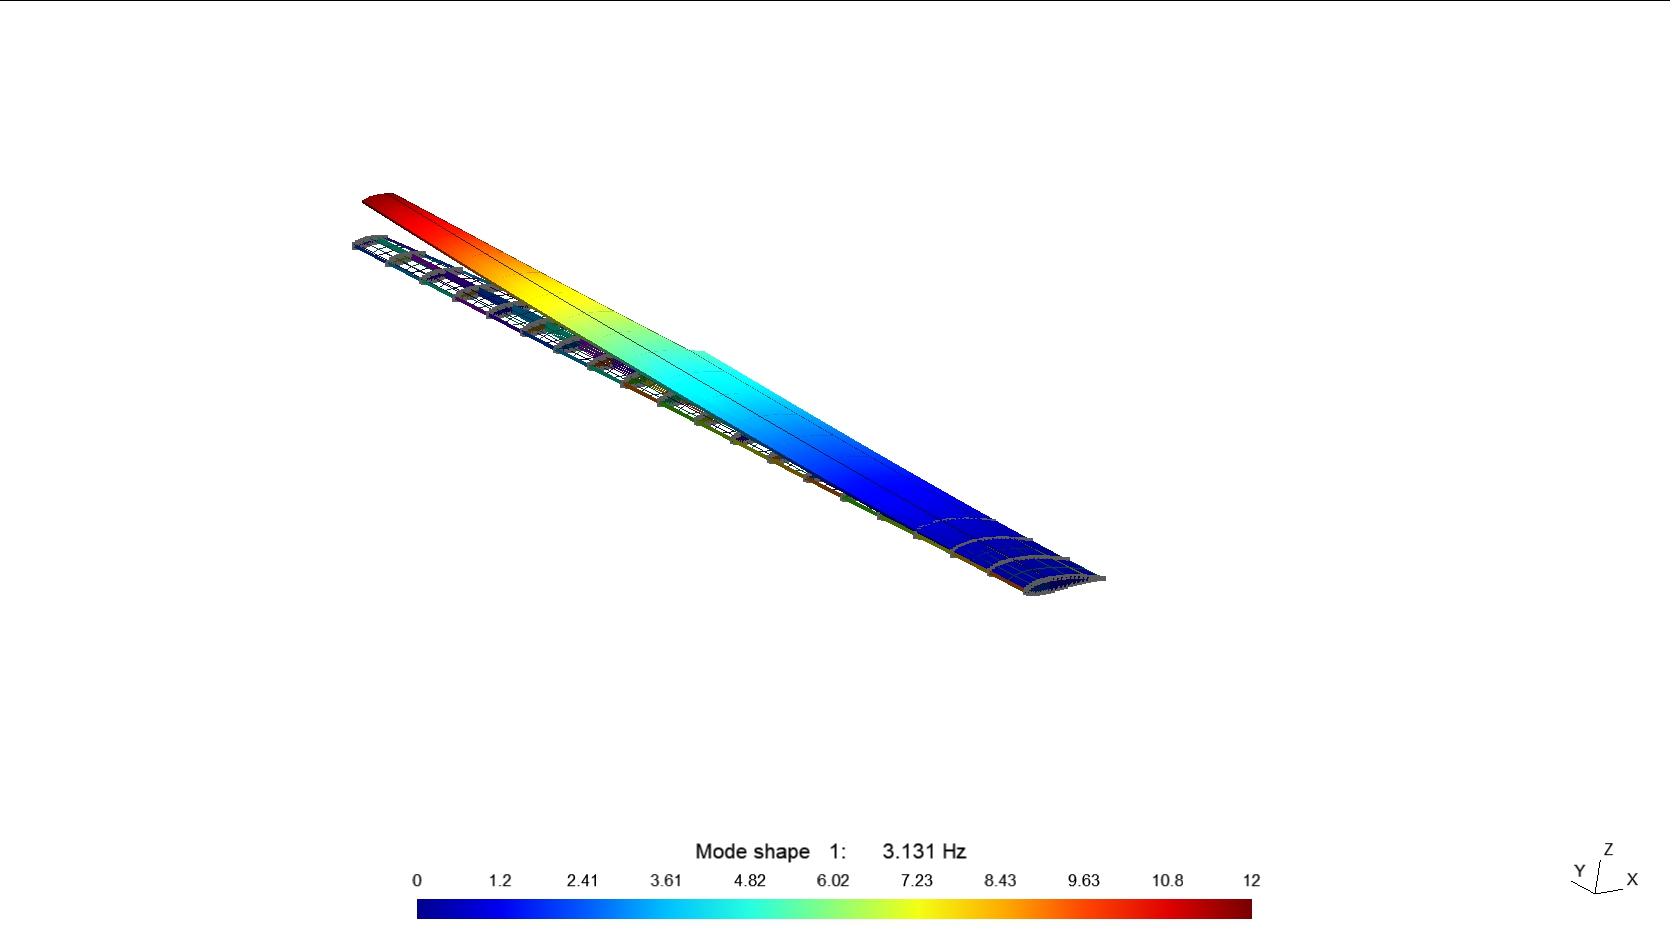
\includegraphics[width=.5\textwidth]{figures/mode1.jpg}
    \caption{The inverse relationship between probability and severity~\cite{CS-25}}
    \label{fig:inverseRelationship}
\end{figure}





\chapter{Code Review}
As in assignment one, the model building of the problem has already been conducted in the statement of the task. Since the solution of the problem is also similar to assignment one, big parts of the code are similar.

The biggest changes in are:

\begin{itemize}
\item A time loop to solve the system of linear equations for each time step
\item Inclusion of a surface plot of the Temperature over time and length
\item Plot of a residual
\item Consideration of $\Delta t$ and density in the source terms
\item Consideration of $\Delta t$ and density in the system matrix
\end{itemize}


\section{Time loop}
\lstinputlisting[language=Matlab, firstline=69, lastline=75, caption={Time loop implementation}, label=lst:timeLoop]{code/main.m}

As seen in \autoref{lst:timeLoop}, a further for loop was implemented in which the system of linear equations is solved in line 2. In line 3, the Temperature over the length is written into the j-th row of T\_time, the source terms are recalculated based on the new Temperature in each cell in line 4 and in line 5 the j-th entry of the residual vector is calculated. Line 6 saves the last Temperature for the next calculation of the residual.


%
\section{Surface plot of T}
\lstinputlisting[language=Matlab, firstline=120, lastline=125, caption={Plotting T over x and t}, label=lst:surfPlot]{code/main.m}

\autoref{lst:surfPlot} shows the implementation of a plot of Temperature over time and x. In line 1 a new figure with id 5 is created, then filled with a surface plot in line 2. Line 3, 4  and 5 set labels for the axes and limits on the time axis.

\section{Plotting the residual}
As already seen in \autoref{lst:timeLoop}, a residual vector is filled every time step. This residual is then plotted over time for every mesh size.


\section{Change to the source terms}
Since the source terms are now dependent on the temperature in each cell and the time step, they are updated each time step. The updated code reflects this dependency as seen in \autoref{lst:sourceTerms} line 9. Also sourceTerms now takes the temperature in each cell, the density and the time step as an input.


\lstinputlisting[language=Matlab, firstline=1, lastline=15, caption={Updated sourceTerms function}, label=lst:sourceTerms]{code/sourceTerms.m}

\section{Change to the system matrix}
The system matrix is now dependent on the time step. This is an additional input argument of the function. It is implemented analogous to sourceTerms.




\chapter{Investigation of mesh size}


Mesh size is investigated for a large amount of time steps and a small time step $\Delta t$. This is so that a time-independent solution is reached. The time step chosen was $\Delta t = 0.01 s$, the end time $t_{end} = 10^4 s$. This is equal to $10^6$ iterations. The mesh sizes chosen were 10, 13, 16, 19, 22, and 25 mesh elements. The error over the length at $t = 10^4 s$ can be seen in \autoref{fig:errT}.


\begin{figure}[H]
    \centering
    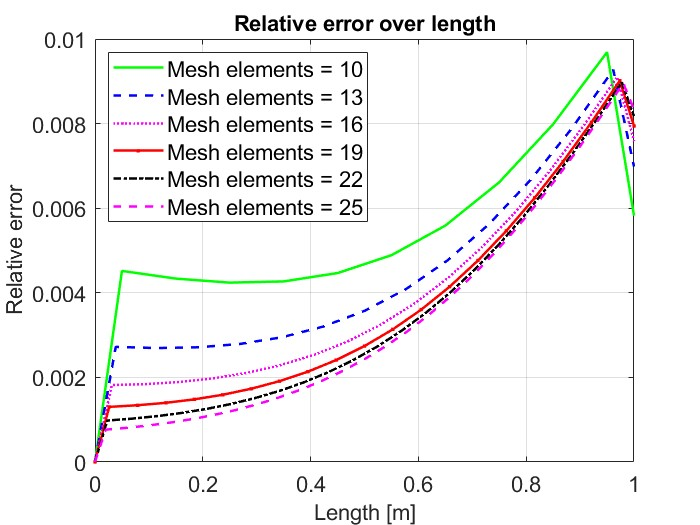
\includegraphics[width=.75\textwidth]{figures/TsmalldtBigtErr.jpg}
    \caption{Relative error to the transient solution over the length of the fin at $t = 10^4 s$}
    \label{fig:errT}
\end{figure}




\begin{figure}[H]
    \centering
    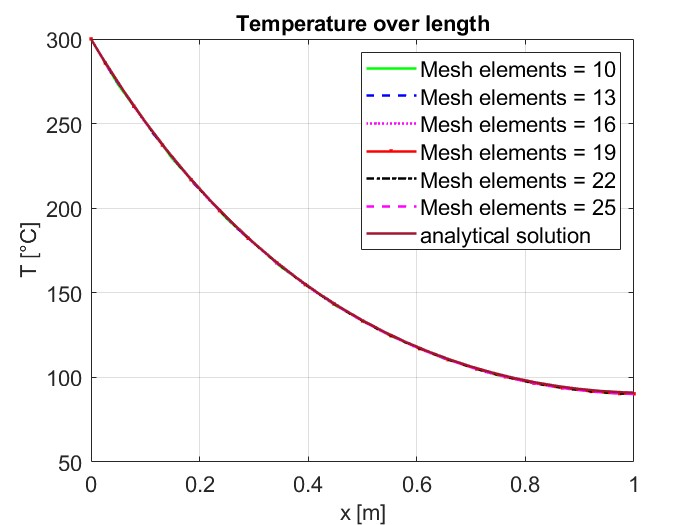
\includegraphics[width=.75\textwidth]{figures/TsmalldtBigt.jpg}
    \caption{Temperature distribution of the transient solution over the length of the fin at $t = 10^4 s$ and the analytical solution}
    \label{fig:T}
\end{figure}

The final temperature distribution as well as the analytical, steady-state solution can be seen in \autoref{fig:T}.

As seen in \autoref{fig:errT} and \ref{fig:T}, the distribution does not depend on mesh size at the chosen time step and end times since the error lies below 1 percent for all meshes, the distributions indistinguishable from the analytical solution. A mesh size of $n = 10$ elements is therefore chosen for further investigations.












\backmatter
\pagenumbering{Roman}


%% --------------------
%% |   Bibliography   |
%% --------------------




%\phantomsection
%\addcontentsline{toc}{chapter}{\bibname}
%\printbibliography[]




%% ----------------
%% |   Appendix   |
%% ----------------

%%%% appendix.tex
%%

\appendix
%\counterwithin{figure}{Abbildungen}
%% ==============================
\chapter{Anhang}
\label{ch:Anhang}
%% ==============================
\section{Abbildungen}
\begin{figure}[H]
    \centering
    \includegraphics[scale=0.22]{text/6mV.jpg}
    \caption{Verlauf von Druck und Geschwindigkeit über Iterationsschritte bei 6m Zellen vor dem Krümmer}
    \label{app:6mV}
\end{figure}

		

\begin{figure}[H]
    \centering
    \includegraphics[scale=0.22]{text/6mN.jpg}
    \caption{Verlauf von Druck und Geschwindigkeit über Iterationsschritte bei 6m Zellen nach dem Krümmer}
    \label{app:6mN}
\end{figure}

\begin{figure}[H]
    \centering
    \includegraphics[scale=0.7]{text/vis.PNG}
    \caption{Visualisierung des Sachverhaltes aus Kapitel~\ref{ch:Parameterstudie}. Geometrie mit 3 Knicken und $l_r = 1$}
    \label{app:vis}
\end{figure}

\begin{figure}[H]
    \centering
    \includegraphics[scale=0.7]{text/mitBlech.png}
    \caption{Strömung im Rohr mit Blech}
    \label{fig:mB}
\end{figure}

\begin{figure}[H]
    \centering
    \includegraphics[scale=0.7]{text/ohneBlech.png}
    \caption{Strömung im Rohr ohne Blech}
    \label{fig:oB}
\end{figure}

\clearpage
\section{Matlab Skripte}

Die hier verwendeten Skripte enthalten Funktionen, die Werte aus surfaceFieldValue.dat importieren. Diese können von Matlab autogeneriert werden und werden hier somit nicht weiter aufgelistet.


\lstset{
  basicstyle=\ttfamily,
  columns=fullflexible,
  frame=single,
  breaklines=true,
  %postbreak=\mbox{\textcolor{blue}{$\hookrightarrow$}\space},
  postbreak=\mbox{\textcolor{red}{>>>}\space},
}


%\captionsetup[lstlisting]{font={small,tt}}
\lstinputlisting[label=app:iterationen,caption=Matlab Skript zum Auftragen von Druck und Geschwindigkeit über die Iterationen,language=Matlab]{text/Iterationen.m}

\clearpage

\lstinputlisting[label=app:comparison,caption=Matlab Skript zum Vergleich verschiedener Simulationsergebnisse,language=Matlab]{text/comparison.m}


\clearpage

\section{OpenFOAM Code}


\lstinputlisting[label=app:sHM,caption=snappyHexMeshDict der Simulation,language=C++]{text/snappyHexMeshDict}%


\clearpage


\lstinputlisting[label=app:bM,caption=blockMeshDict der Simulation,language=C++]{text/blockMeshDict}%


\clearpage

\lstinputlisting[label=app:av,caption=Fläche über welche ein Mittelwert gebildet wird,language=C++]{text/average_01}



%%\nomenclature{\rho}{Dichte [$\frac{kg}{m^3}$]}



\end{document}
